\documentclass{beamer}
\usepackage[utf8]{inputenc}

\usetheme{Madrid}
\usecolortheme{default}
\usepackage{extarrows}
\usepackage{amsmath}
\usepackage{extarrows}
\usepackage{amssymb,amsfonts,amsthm}
\usepackage{txfonts}
\usepackage{tkz-euclide}
\usepackage{listings}
\usepackage{adjustbox}
\usepackage{array}
\usepackage{tabularx}
\usepackage{gvv}
\usepackage{lmodern}
\usepackage{circuitikz}
\usepackage{tikz}
\usepackage{graphicx}
\usepackage{amsmath} 

\setbeamertemplate{page number in head/foot}[totalframenumber]

\usepackage{tcolorbox}
\tcbuselibrary{minted,breakable,xparse,skins}

\definecolor{bg}{gray}{0.95}
\DeclareTCBListing{mintedbox}{O{}m!O{}}{%
  breakable=true,
  listing engine=minted,
  listing only,
  minted language=#2,
  minted style=default,
  minted options={%
    linenos,
    gobble=0,
    breaklines=true,
    breakafter=,,
    fontsize=\small,
    numbersep=8pt,
    #1},
  boxsep=0pt,
  left skip=0pt,
  right skip=0pt,
  left=25pt,
  right=0pt,
  top=3pt,
  bottom=3pt,
  arc=5pt,
  leftrule=0pt,
  rightrule=0pt,
  bottomrule=2pt,
  toprule=2pt,
  colback=bg,
  colframe=orange!70,
  enhanced,
  overlay={%
    \begin{tcbclipinterior}
    \fill[orange!20!white] (frame.south west) rectangle ([xshift=20pt]frame.north west);
    \end{tcbclipinterior}},
  #3,
}
\lstset{
    language=C,
    basicstyle=\ttfamily\small,
    keywordstyle=\color{blue},
    stringstyle=\color{orange},
    commentstyle=\color{green!60!black},
    numbers=left,
    numberstyle=\tiny\color{gray},
    breaklines=true,
    showstringspaces=false,
}
\title %optional
{4.11.10}
\date{September 13 ,2025}

\author 
{Kartik Lahoti - EE25BTECH11032}

\begin{document}


\frame{\titlepage}
\begin{frame}{Question}
Point $\vec{A}$ lies on the line segment $\vec{XY}$  joining $\vec{X}\brak{6,-6}$ and $\vec{Y}\brak{-4,-1}$ in such a way that $\frac{\vec{XA}}{\vec{XY}} = \frac{2}{5}$. if point $\vec{A}$ also lies on the line $3x + k(y+1) = 0$, find the value of $k$ .
\end{frame}

\begin{frame}{Theoretical Solution}

\begin{table}[H]
    \centering
    \begin{table}[h!]
    \centering
    \begin{tabular}{|c|c|}
        \hline
        Point & Coordinates \\
        \hline
	    $A$ & $\myvec{1\\-1}$ \\
	    $B$ & $\myvec{-4\\2k}$ \\
	    $C$ & $\myvec{-k\\-5}$ \\
        \hline
    \end{tabular}
    \caption{Vertices of $\triangle ABC$ before substituting $k$}
    \label{tab:triangle_k}
\end{table}

    \caption{4.11.10}
    \label{tab:placeholder_1}
\end{table}

Given Line Equation, 

\begin{align}
        \myvec{3 & k}\myvec{x \\ y} + k &= 0  
\end{align}

\end{frame}
\begin{frame}{Theoretical Solution}

\begin{align}
    \frac{\vec{XA}}{\vec{XY}} &= \frac{2}{5}\\ 
    \frac{\vec{XA}}{\vec{XY}-\vec{XA}} &= \frac{2}{5-2} \\
    \frac{\vec{XA}}{\vec{YA}} &= \frac{2}{3} 
\end{align}

Using Section Formula, 
\begin{align}
  \vec{A} =  \frac{1}{1 + \frac{2}{3}}\brak{\myvec{6 \\ -6} + \frac{2}{3}\myvec{-4\\-1}} = \myvec{2 \\ -4}
\end{align}

\end{frame}
\begin{frame}{Theoretical Solution}

Putting $\vec{A}$ in the given line equation,
\begin{align}
  \myvec{3 & k}\myvec{2 \\ -4 } + k &= 0 
\end{align}
\begin{align}
    6 - 4k + k &= 0 
\end{align}
\begin{align}
    k &= 2
\end{align}
\end{frame}

\begin{frame}{Theoretical Solution}
Hence, 
\begin{align}
  \vec{A} = \myvec{2 \\ -4} \text{ and } k = 2
\end{align}
\end{frame}

\begin{frame}[fragile]
    \frametitle{C Code (1)}

    \begin{lstlisting}
void section_formula ( double *X , double *Y , double *A , double ratio , int m  )
{
    for(int i = 0;  i < m ; i++)	
	A[i] = (1/(1+ratio))*(X[i] + ratio * Y[i] );
}
    \end{lstlisting}
\end{frame}

\begin{frame}[fragile]
    \frametitle{C Code (2) - Function to Generate Points on Line}
    \begin{lstlisting}
    
void linegen(double *XY, double *A , double *B , int n , int m )
{
    double temp[m] ; 
    for (int i = 0 ; i < m ; i++)
    {
        temp [ i ] = (B[i]- A[i]) /(double) n ; 
    }
    for (int i = 0 ; i < n ; i++ )
        for (int j = 0 ; j < m ; j++)
            XY[j*n + i ] = A[j] + temp[j] * i ; 
           
}

\end{lstlisting}
\end{frame}

\begin{frame}[fragile]
    \frametitle{Python Code - Using Shared Object}
    \begin{lstlisting}
import ctypes as ct
import numpy as np
import matplotlib.pyplot as plt

handc1 = ct.CDLL("./func.so")

handc1.section_formula.argtypes = [
    ct.POINTER(ct.c_double),
    ct.POINTER(ct.c_double),
    ct.POINTER(ct.c_double),
    ct.c_double,
    ct.c_int
]
handc1.section_formula.restype = None

\end{lstlisting}
\end{frame}

\begin{frame}[fragile]
    \frametitle{Python Code - Using Shared Object}
    \begin{lstlisting}

X = np.array([6,-6] , dtype = np.float64).reshape(-1,1)
Y = np.array([-4,-1] , dtype = np.float64).reshape(-1,1)
A = np.zeros(2, dtype = np.float64).reshape(-1,1)
p = 2 / 3 
handc1.section_formula(
    X.ctypes.data_as(ct.POINTER(ct.c_double)),
    Y.ctypes.data_as(ct.POINTER(ct.c_double)),
    A.ctypes.data_as(ct.POINTER(ct.c_double)),
    p , 2
)
print("Vector A = ",A)

\end{lstlisting}
\end{frame}

\begin{frame}[fragile]
    \frametitle{Python Code - Using Shared Object}
    \begin{lstlisting}
M = np.array([-10,14] , dtype = np.float64).reshape(-1,1)
N = np.array([10,-16] , dtype = np.float64).reshape(-1,1)

def line(P: np.ndarray , Q: np.ndarray, str1 , str2):
    handc2 = ct.CDLL("./line_gen.so")

    handc2.linegen.argtypes = [
        ct.POINTER(ct.c_double),
        ct.POINTER(ct.c_double),
        ct.POINTER(ct.c_double),
        ct.c_int , ct.c_int
    ]
    handc2.linegen.restype = None
    
\end{lstlisting}
\end{frame}
\begin{frame}[fragile]
    \frametitle{Python Code - Using Shared Object}
    \begin{lstlisting}
    n = 200
    XY = np.zeros((2,n),dtype=np.float64)

    handc2.linegen (
        XY.ctypes.data_as(ct.POINTER(ct.c_double)),
        P.ctypes.data_as(ct.POINTER(ct.c_double)),
        Q.ctypes.data_as(ct.POINTER(ct.c_double)),
        n,2
    )
    plt.plot(XY[0,:],XY[1,:], str1 , label = str2 )
    \end{lstlisting}
\end{frame}

\begin{frame}[fragile]
    \frametitle{Python Code - Using Shared Object}
    \begin{lstlisting}
plt.figure()

line(X,Y,"g--","Line Segment XY")
line(M,N,"r-","Line Containing A")
coords = np.block([[X,Y,A]])

plt.scatter(coords[0,:] , coords[1,:])
vert_label = ['X', 'Y' , 'A' ]

for i , txt in enumerate(vert_label) :
    plt.annotate(f"{txt}\n({coords[0,i]:.1f},{coords[1,i]:.1f})",
                 (coords[0,i], coords[1,i]),
                 textcoords = "offset points" ,
                 xytext = (0,-30),ha = "center")
\end{lstlisting}
\end{frame}

\begin{frame}[fragile]
    \frametitle{Python Code - Using Shared Object}
    \begin{lstlisting}
plt.xlim([-6,8])
plt.ylim([-8,0])
plt.xlabel("$x$")
plt.ylabel("$y$")
plt.grid()

plt.legend(loc="best")

plt.title("4.11.10")

plt.savefig("../figs/section1.png")
plt.show()

#plt.savefig('../figs/section1.png')
#subprocess.run(shlex.split("termux-open ../figs/section1.png"))

\end{lstlisting}
\end{frame}

\begin{frame}[fragile]
    \frametitle{Python Code}
    \begin{lstlisting}
mport math
import sys 
sys.path.insert(0, '/home/kartik-lahoti/matgeo/codes/CoordGeo')
import numpy as np
import numpy.linalg as LA
import matplotlib.pyplot as plt

from line.funcs import *

#if using termux
#import subprocess
#import shlex
\end{lstlisting}
\end{frame}

\begin{frame}[fragile]
    \frametitle{Python Code }
    \begin{lstlisting}
X = np.array([6,-6] , dtype = np.float64).reshape(-1,1)
Y = np.array([-4,-1] , dtype = np.float64).reshape(-1,1)
k = 2 / 3
A = (1/(1+k))*(X + k * Y)
 
print("Vector A = " , A ) 

M = np.array([-10,14] , dtype = np.float64).reshape(-1,1)
N = np.array([10,-16] , dtype = np.float64).reshape(-1,1)
\end{lstlisting}
\end{frame}

\begin{frame}[fragile]
    \frametitle{Python Code }
    \begin{lstlisting}
def plot_it(P,Q,str1,str2):
    x_l = line_gen_num(P,Q,20)
    plt.plot(x_l[0,:],x_l[1,:] , str1 , label =  str2)

plt.figure()

plot_it(X,Y,"g--","Line Segment XY")
plot_it(M,N,"r-","Line Containing A")
coords = np.block([[X,Y,A]])
plt.scatter(coords[0,:],coords[1,:])
vert_labels = ['X','Y','A']


\end{lstlisting}
\end{frame}

\begin{frame}[fragile]
    \frametitle{Python Code }
    \begin{lstlisting}

for i, txt in enumerate(vert_labels):
    plt.annotate(f'{txt}\n({coords[0,i]:.1f}, {coords[1,i]:.1f})',
                 (coords[0,i], coords[1,i]),
                 textcoords="offset points",
                 xytext=(0,-30),
                 ha='center')
                 
    \end{lstlisting}
\end{frame}
\begin{frame}[fragile]
    \frametitle{Python Code }
    \begin{lstlisting}
    
plt.xlim([-6,8])
plt.ylim([-8,0])
plt.xlabel('$x$')
plt.ylabel('$y$')
plt.grid()
plt.legend(loc = "best")
plt.title("Fig:4.11.10")
plt.savefig("../figs/section2.png")
plt.show()

#plt.savefig('../figs/section1.png')
#subprocess.run(shlex.split("termux-open ../figs/section1.png"))

    \end{lstlisting}
\end{frame}


\begin{frame}{Plot}
    \centering
    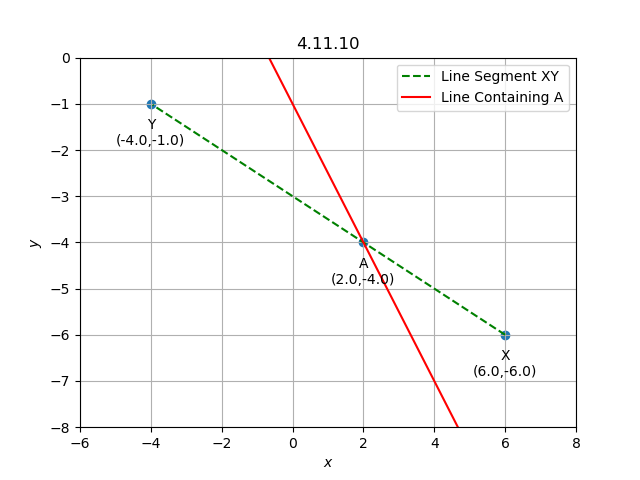
\includegraphics[width=\columnwidth, height=0.8\textheight, keepaspectratio]{../figs/section1.png}   
\end{frame}

\end{document}
